\documentclass[tikz,border=10pt]{standalone}
\begin{document}
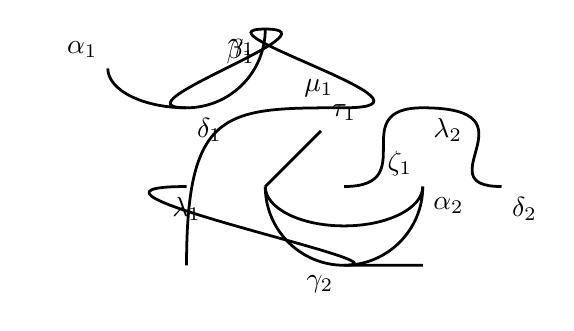
\begin{tikzpicture}[line width=1pt]
% Draw the curves
\draw (0,0) .. controls ++(90:2) and ++(180:1.5) .. (2,2) coordinate (mu1)
.. controls ++(0:1.5) and ++(180:1) .. (1,3) coordinate (gamma1)
.. controls ++(0:1) and ++(180:1) .. (0,2) coordinate (delta1);

\draw (2,1) .. controls ++(0:1) and ++(180:1) .. (3,2) coordinate (lambda2)
.. controls ++(0:1.5) and ++(180:1) .. (4,1) coordinate (delta2);

\draw (3,0) .. controls ++(180:1.5) and ++(0:1) .. (2,0) coordinate (gamma2)
.. controls ++(0:1) and ++(180:2) .. (0,1) coordinate (lambda1);

% Draw the arcs
\draw (1,1) arc (180:360:1cm) coordinate (alpha2);
\draw (1,1) arc (180:360:1cm and .5cm) coordinate (zeta1);
\draw (1,1) -- ++(45:1cm) coordinate (tau1);

\draw (0,2) arc (270:360:1cm) coordinate (beta1);
\draw (0,2) arc (270:180:1cm and .5cm) coordinate (alpha1);

% Label the points
\node[above left] at (mu1) {$\mu_1$};
\node[below left] at (gamma1) {$\gamma_1$};
\node[below right] at (delta1) {$\delta_1$};

\node[below right] at (lambda2) {$\lambda_2$};
\node[below right] at (delta2) {$\delta_2$};
\node[below left] at (gamma2) {$\gamma_2$};

\node[below] at (lambda1) {$\lambda_1$};
\node[below left] at (beta1) {$\beta_1$};
\node[below right] at (alpha2) {$\alpha_2$};
\node[above left] at (zeta1) {$\zeta_1$};
\node[above right] at (tau1) {$\tau_1$};
\node[above left] at (alpha1) {$\alpha_1$};
\end{tikzpicture}
\end{document}